\documentclass[9pt,notheorems]{beamer} %global font-size
\usepackage{UESTC}

\usepackage{hyperref}
\usepackage[T1]{fontenc}
\usepackage{latexsym,amsmath,xcolor,multicol,booktabs,calligra}
\usepackage{graphicx,pstricks,listings,stackengine}
\usepackage[linesnumbered,ruled,vlined]{algorithm2e}
\usepackage{multirow}
\usepackage{pgfpages}

\author{mobbu}
\title{How To Make An Academic PPT}
\subtitle{Graduation Project Proposal Report}
\institute{CSIS in UESTC}
\date{\today}

\begin{document}

\begin{frame}
    \titlepage
    \begin{figure}[htpb]
        \begin{center}
            
\includegraphics[width=0.2\linewidth]{pic/logo.pdf}
        \end{center}
    \end{figure}
\end{frame}

\begin{frame}
    \tableofcontents[sectionstyle=show,subsectionstyle=show/shaded/hide,subsubsectionstyle=show/shaded/hide]
\end{frame}

\section{kun}
\begin{frame}{this is kunkun}
    this is kun play basketball
    \begin{figure}
        \only<1>{
            \begin{center}
                
\includegraphics[width=0.8\linewidth]{pic/01.jpg}
            \end{center}
        }
        \only<2>{
            \begin{center}
                
\includegraphics[width=0.8\linewidth]{pic/02.jpg}
            \end{center}
        }
        \only<3>{
            \begin{center}
                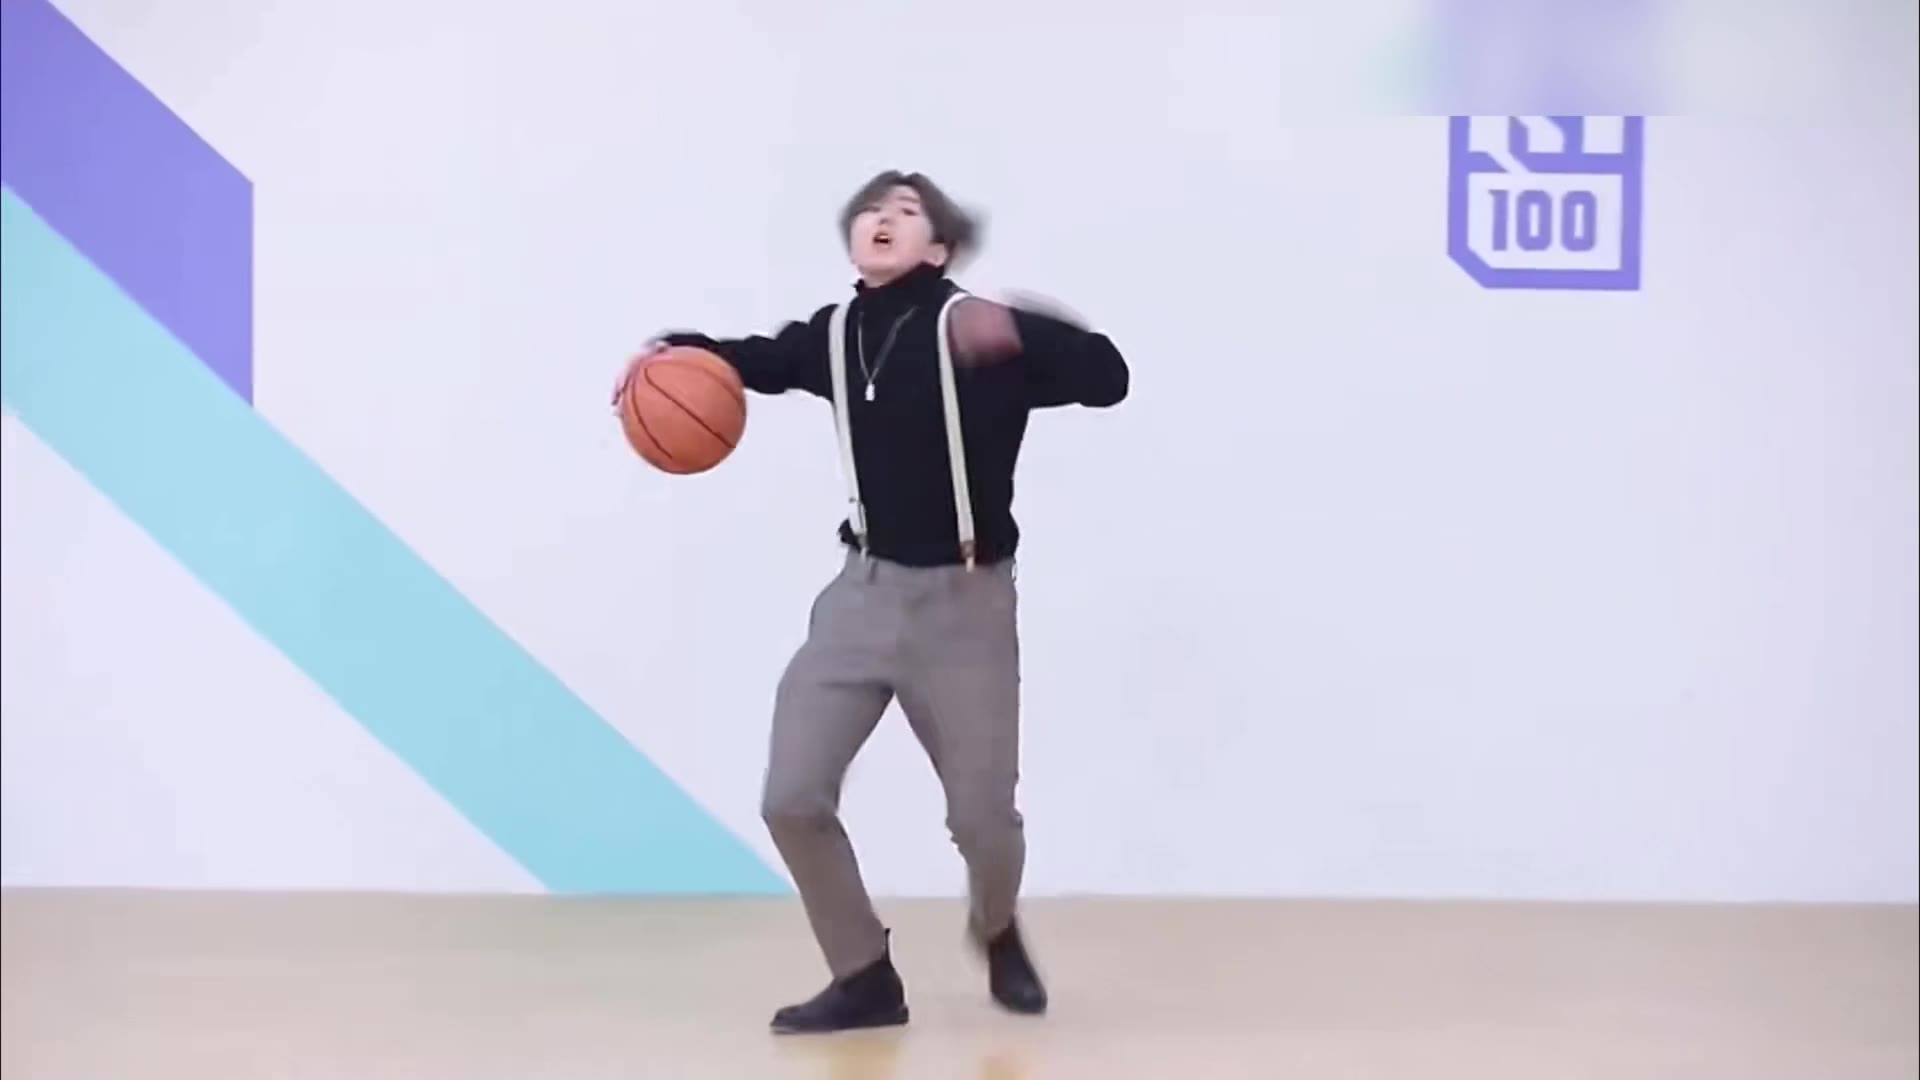
\includegraphics[width=0.8\linewidth]{pic/03.jpg}
            \end{center}
        }
        \only<4>{
            \begin{center}
                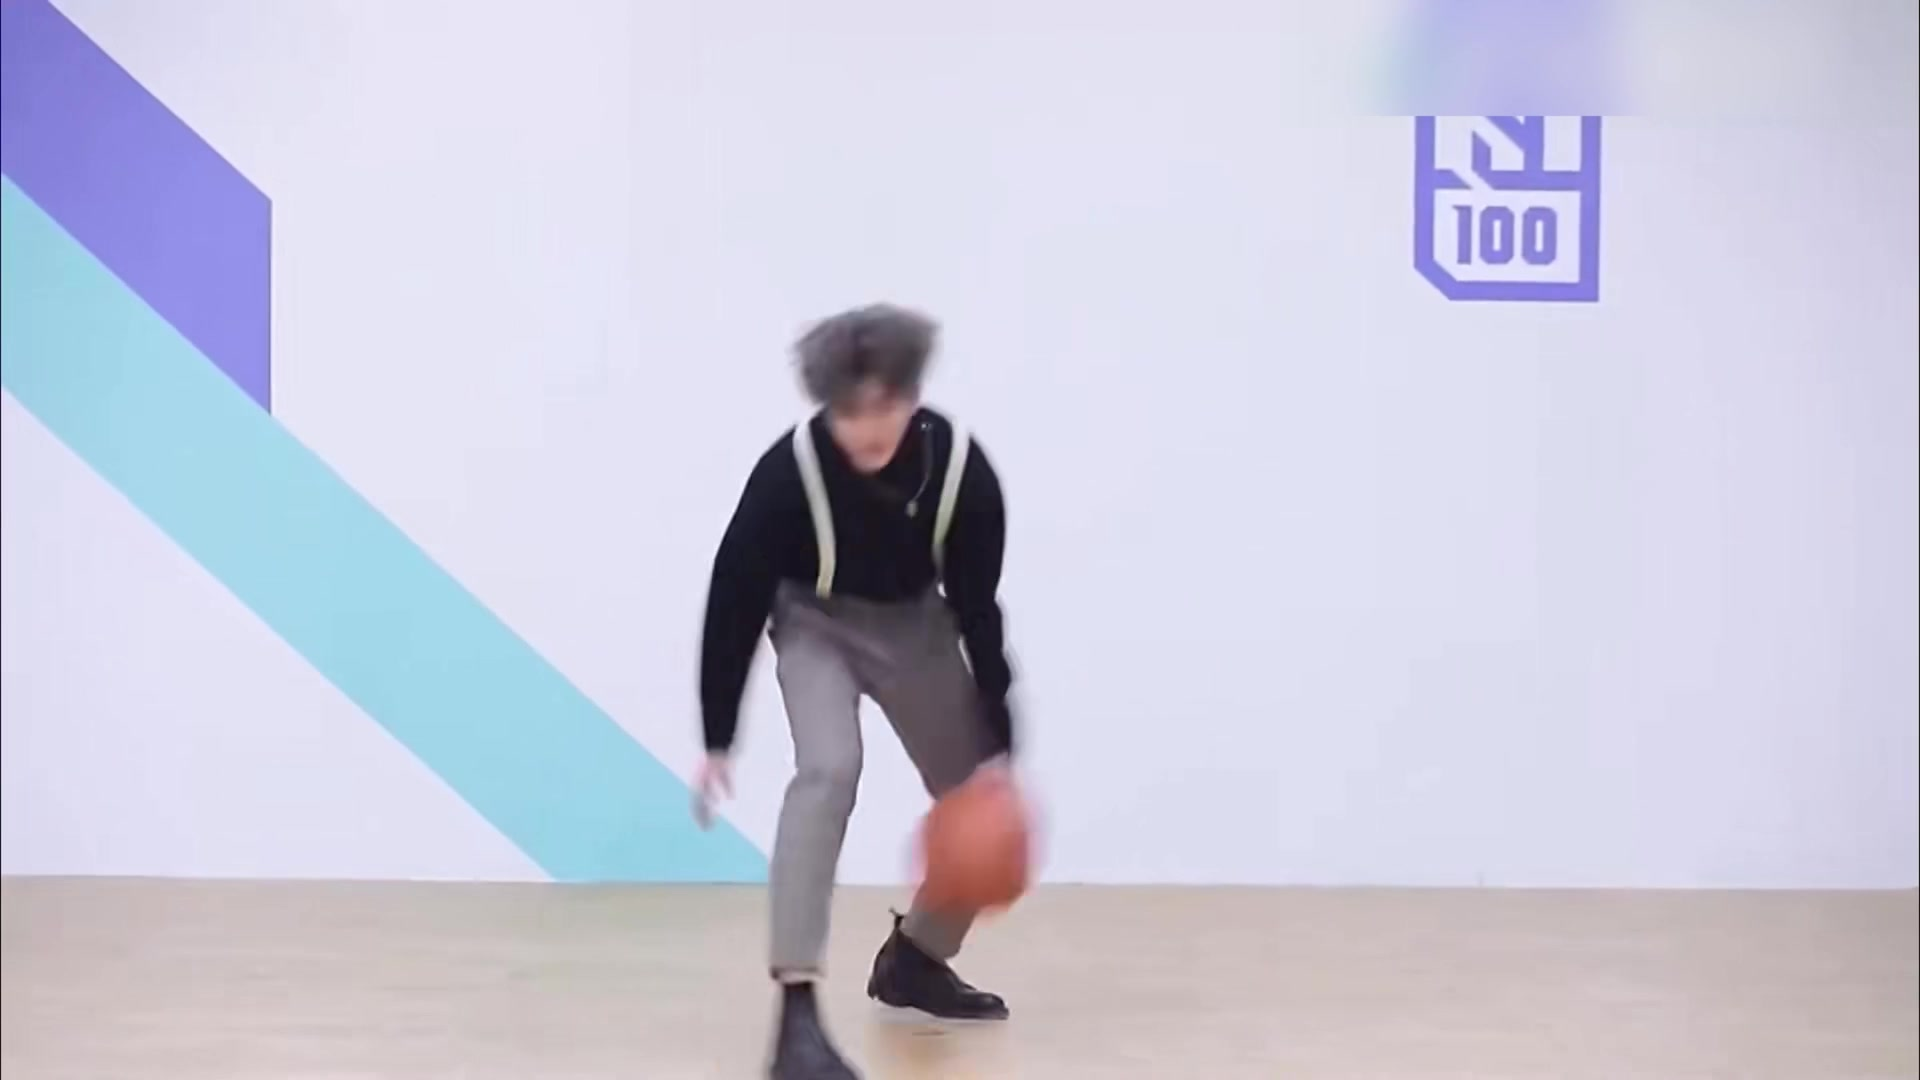
\includegraphics[width=0.8\linewidth]{pic/04.jpg}
            \end{center}
        }
        \caption{ikun.}
    \end{figure}

\end{frame}

\end{document}